
\section{Datafari}

\subsection{Installation}

Für Datafari musste folgende Software nachinstalliert werden: Java 8 und JQ, ein JSON-Prozessor. Damit die Installation richtig durchläuft, muss die JAVA\_HOME-Variable erstellt werden. Insofern Datafari nicht unter Root laufen soll, muss noch ein besonderer Nutzer mit Root Rechten angelegt werden. Dieser muss wie schon bei Solr höhere User-Limits erhalten. Datafari installiert sich selbst durch eine DEB-Datei. Während der Installation erscheint ein kurzer Setup-Dialog, welcher einen durch die Konfiguration führt. Das Starten des Server geschieht daraufhin durch ein Script im Installationsordner.

\subsection{Indexierung}

Damit eine Indexierung durchgeführt werden kann, muss bei Datafari ein sogenanntes Repository angelegt werden. In diesem wird die Datenbank-Verbindung eingetragen. Dabei ist es wichtig, dass vorher der Treiber korrekt installiert wird. Es kam bei mir dabei zu Problemen. 
Das auf Apache ManifoldCF basierende System akzeptiert nur MySQL-JDBC Treiber. Da der MariaDB-Treiber einen anderen Klassennamen in Java verwendet, funktioniert dieser nicht. \begin{quote} This connection type cannot be configured to work with other databases than the ones listed above without software changes.~\cite[S.~61]{ApacheSoftwareFoundation.}\end{quote} Deswegen musste ich für diesen Test den MySQL-Treiber von Oracle verwendet.
Nachdem der Treiber korrekt installiert ist und das Repository erstellt ist, kann nun einen Job zu Indexierung der Einträge starten. In dem werden die Queries und der Zeitplan konfiguriert.
CONTINUE HERE!

\subsection{Oberfläche}

Die Oberfläche von Datafari ist dreigeteilt. Zum einen gibt eine Such-Oberfläche, welche sich ohne Anmeldung erreichen lässt. Als Zweites findet sich eine Administrationsoberfläche, welche erst eingesehen werden kann, sobald man eingeloggt ist. Dort findet man diverse Einstellungen für die Suchmaschinen, wie Synonyme oder die Facetten-Konfiguration. Auch sind dort die Logs einzusehen, welche durch die Einbindung der Oberfläche von Kibana \ref{elasticsearch} aus ELK-Stack angezeigt werden. Die dritte Oberfläche ist die Einstellungsseite für die Datacrawler. Dies ist eine modifizierte Oberfläche von Apache ManifoldCF. Generell sind die Menüs sehr übersichtlich, auch wenn die Einbindung von anderen Anwendungen keine Ideale Lösung darstellt. Es lassen sich keine Updates direkt über die Oberfläche einspielen.
!!CONTINUE RESPONSIVE UND UPDATES!!

\subsection{Dokumentation}

Die Dokumentation geht sehr genau auf die Installation des Systems ein, dabei werden alle Konfigurationsaspekte beleuchtet. Zum Beispiel wird beschrieben, wie die User Limits erhöht werden, oder die JAVA\_HOME-Variable korrekt gesetzt wird. Allerdings merkt man an manchen Stellen, dass die Dokumentation nicht von nativen Englischsprechenden geschrieben wurde, da die Grammatik nicht immer stimmt. Allerdings hat dies nie zu Problemen oder Verwechslungen geführt.
Bei der Dokumentation zum Einrichten des JDBC-Treibers finden sich einige Probleme \ref{img:datafariJDBC}. Zum einen sind beide Pfade, die in dem Text angegeben sind, falsch. Einer davon wird sogar richtig in dem Screenshot direkt darunter angezeigt. Und zum anderen ist der zweite Screenshot so niedrig aufgelöst, dass sich nicht viel erkennen lässt. Dies passiert auch, wenn das Bild in einen neuen Tab geladen wird. Generell ist die Dokumentation für den Umgang mit Datenbanken nicht sehr ausführlich. Die Erklärungen, wofür die Variables bei der Erstellung eines Jobs stehen, musste ich in der Dokumentation von ManifoldCF nachlesen.
Die Dokumentation ist im aktuellen Stand nicht sauber strukturiert. Sie gibt das Gefühl, dass es sich eher um eine Sammlung verschiedener Artikel, welche Intern genutzt wurden, handelt.

\begin{figure}
	\centering
	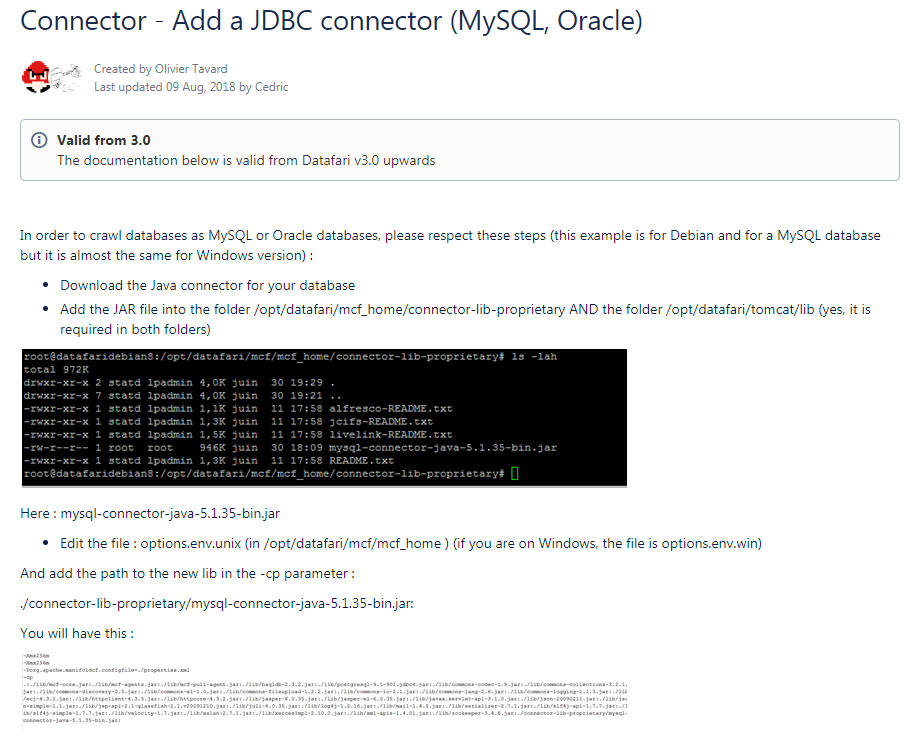
\includegraphics[width=1\linewidth]{images/datafari_doku_wrong_path.png}
	\caption{Dokumentationsseite für den JDBC Treibers von Datafari.}
	\label{img:datafariJDBC}
\end{figure}


\subsection{Absetzen einer Anfrage und Integration in PHP}
